%! TEX root = **/010-main.tex
% vim: spell spelllang=ca :

\section{Codis de MATLAB}

\subsection{Preprocessat}%
\label{app:pre}

\inputminted{matlab}{./code/preprocess.m}

\subsection{Shape Signature}%
\label{app:shapesig}
\inputminted{matlab}{./code/shapeSignature.m}

\pagebreak
\subsection{Color}%
\inputminted{matlab}{./code/splitColor.m}

\section{Resultats}%
\label{app:exemple}

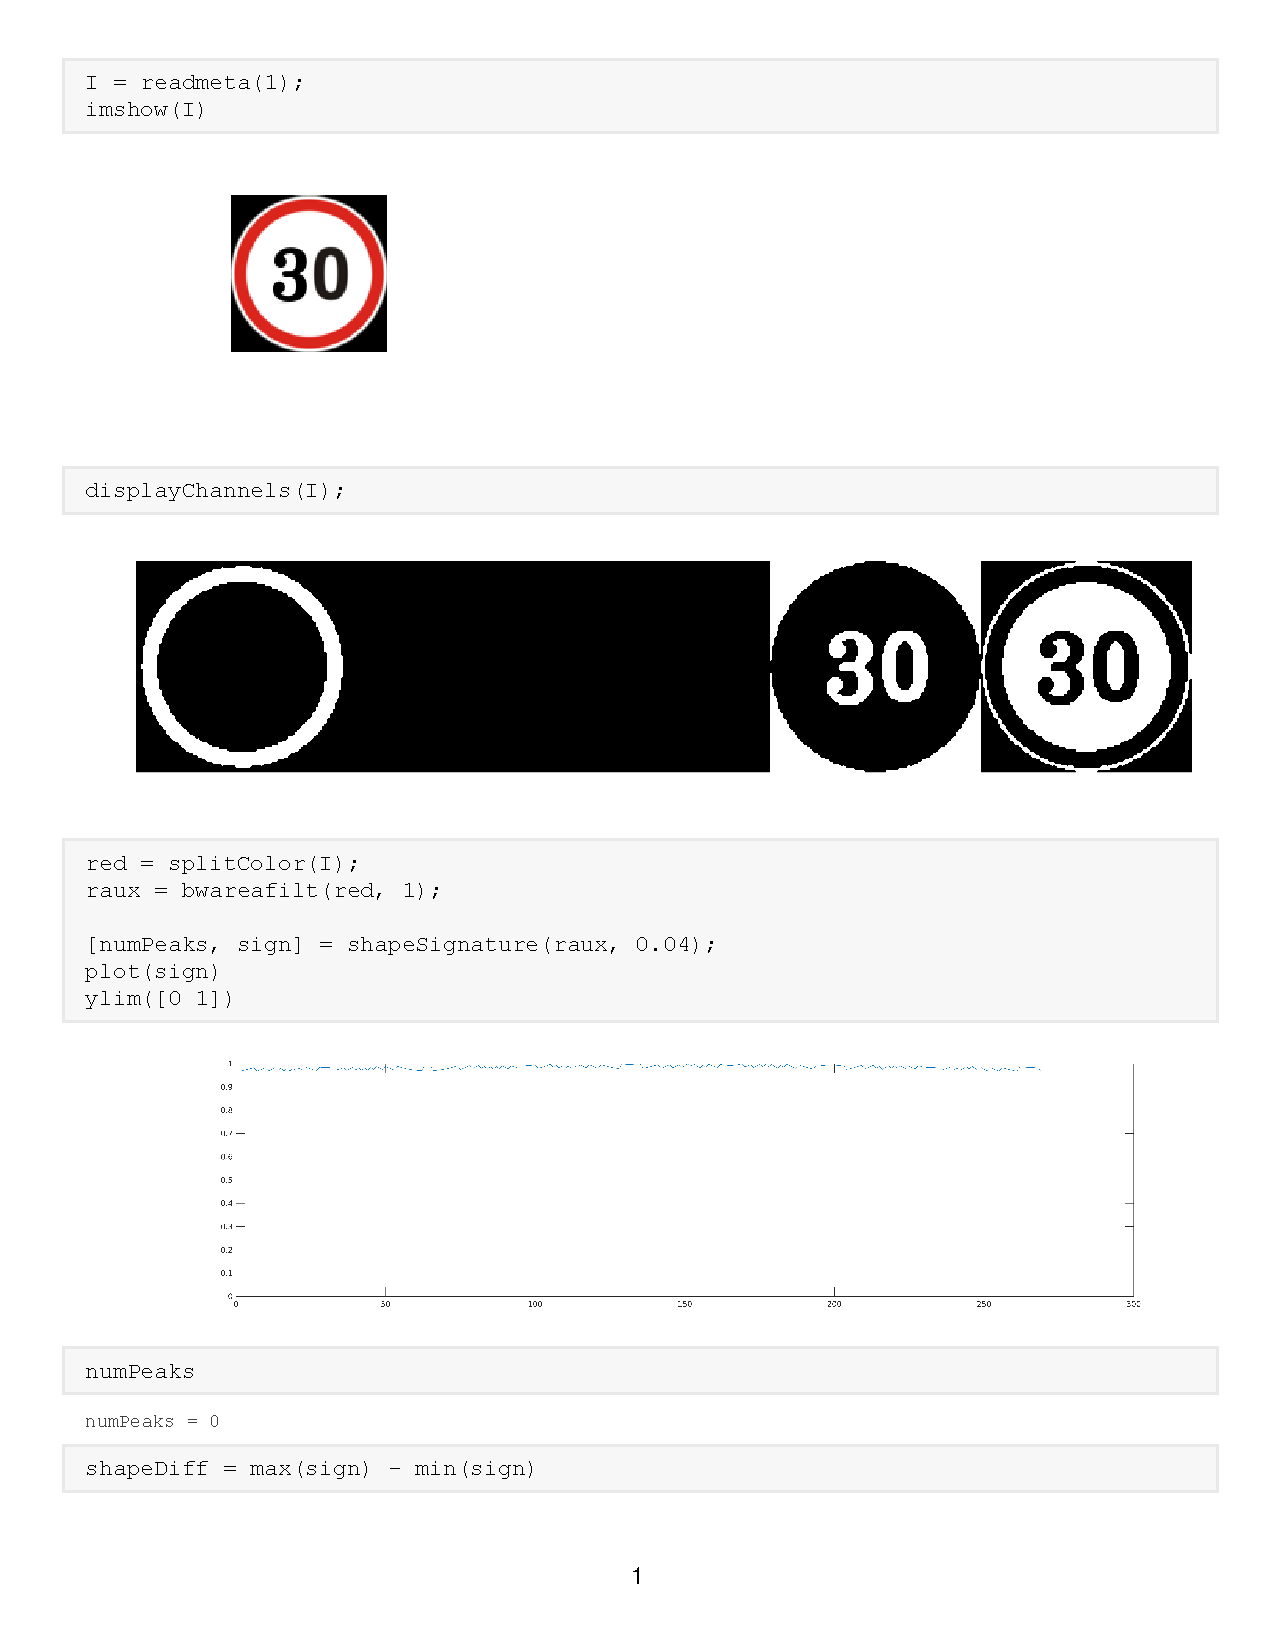
\includepdf[pages={1-5}]{test.pdf}
